\documentclass{article}
\usepackage{graphicx} % Required for inserting images
\usepackage[margin=2.5cm]{geometry} % Configura todos los márgenes a 2.5 cm
\usepackage{setspace}
\onehalfspacing % Interlineado de 1.5 % \doublespacing % Interlineado doble
\usepackage{float}

\title{Super Mario el inicio de una gran saga de los videojuegos}
\author{Luis Angel Cruz Hernandez}
\date{September 2026}

\begin{document}

\maketitle

\section{Super Mario Bros}

Para empezar, conozcamos un poco la historia detrás de esta gran saga, en aquel 1985 donde saldría el primer \textit{"Super Mario Bros"} sacado en la consola de \textbf{NES}, el cual revoluciono el mundo de los videojuegos en su época, porque era cuando el mundo de los videojuegos estaba pasando por una muy mala racha, se puede decir que Nintendo salvo la industria de los videojuegos en su momento, pero bueno centrándonos más en Mario Bros, este tiene alta referencia por ser uno de los pioneros en tener un personaje característico, que más tarde sería la gran mascota de Nintendo que en mucho tiempo no lograron ni llegarle a los talones, esto empieza con su primer juego \textbf{"Super Mario Bros"}, donde fue el boom, un juego de plataformas que tendría una jugabilidad simple, divertida y niveles perfectamente diseñados que conquistaron al mundo, esto fue el boom en la industria, ya que nuevamente se veía a los videojuegos diferentes y le daban una gran importancia, después de tener una mala racha, volvían a renacer como un ave fénix, donde Nintendo hizo que los videojuegos volvieran a ser muy relevantes en 1985.

\begin{figure}[H]
    \centering
    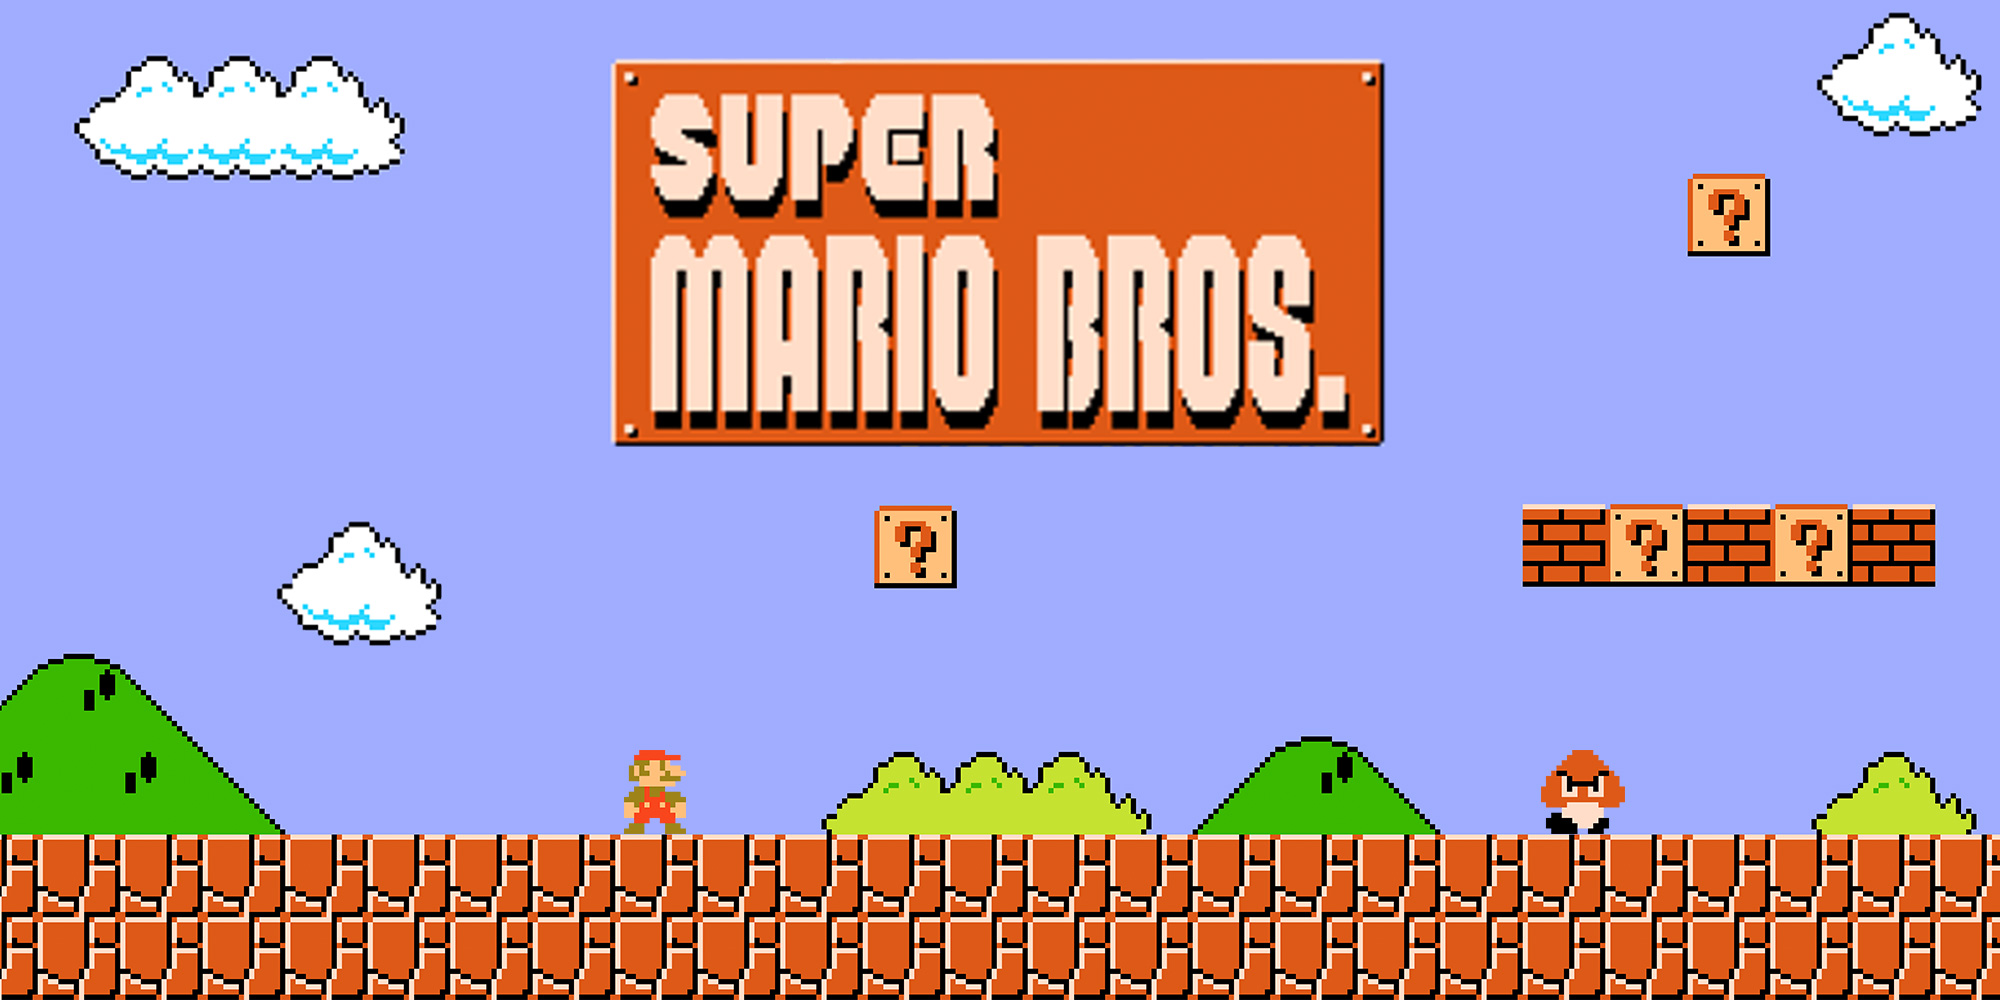
\includegraphics[width=1\linewidth]{image1.png}
    \caption{Super Mario Bros}
    \label{fig:placeholder1}
\end{figure}

\newpage

\section{El comienzo de una gran era}

Continuando, Nintendo tras apostar por lanzar este videojuego, empezó a sacar más videojuegos muy característicos que igual alcanzaron una gran fama, como puede ser el \textbf{The legend of Zelda, Kirby, Pokemon, Metroid}, entre otros. Estos siendo igualmente muy importante y siendo cada uno una de las grandes joyas de la consola \textbf{NES}, pero esto hizo que nintendo se diera cuenta que Mario tenía grandes proyecciones para futuro, después del gran impacto que hizo, sacaron otro Super Mario Bros, el cual fue el \textbf{"Super Marios Bros The lost levels"}, este siendo considerado muy difícil por los japoneses, esto hizo que sacaran otra versión para Norteamérica que sería el \textit{"Super Marios Bros 2"}, el cual decían que era más fácil y muy diferente a la que ya venían trabajando con the lost levels, pero lo bueno fue que vino después el gran y tan ansiado \textit{"Super Mario Bros 3"}, el cual fue la tercera de nuestro fontanero favorito, este videojuego como tal fue creado por 20 y 30 personas que operaban en Nintendo, siendo algo muy increíble por lo bien que estaba desarrollado el juego, con una increíble calidad de niveles, de diseños y sobre todo entretenido para el jugador, esto hizo que despegara por mucho Nintendo y más en concreto la saga de \textit{"Super Mario Bros"}, ya que después de todo volvieron más fuertes que nunca, ya que el próximo en  lanzarse fue el \textbf{"Super Mario Bros World"}, siendo este también un gran exitaso en todo su esplendor, y siguieron y siguieron sacando buenos juegos de Super Mario, volviendo así a Super Mario Bros una de las grandes sagas de todos los videojuegos y siendo vigente hasta los últimos años, la gran parte del fandom e incluyéndome estamos en la espera que Nintendo anuncie el próximo Mario 3D que es algo muy esperado desde el 2019.

\begin{figure}[H]
    \centering
    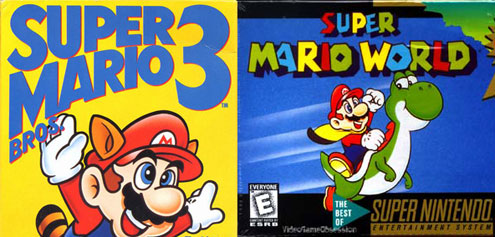
\includegraphics[width=1\linewidth]{image2.png}
    \caption{Mario 3 y Mario World}
    \label{fig:placeholder2}
\end{figure}

\newpage

Otros grande titulos de Super Mario Bros que saco Nintendo fueron:
\begin{itemize}
    \item Super Mario 64
    \item Super Mario Galaxy
    \item New Super Mario Bros WII
    \item Super Mario Bros Wonder
    \item Super Mario Maker
    \item Super Mario Galaxy
    \item Super Mario 3D World
    \item Super Mario Sunshine
    \item Super Mario ALL STARS
\end{itemize}

\section{Referencias}

\begin{itemize}
    \item ALVY.(2016).1983: el año en que ¿murieron? los videojuegos.
    \\Recuperado de:\\https://www.microsiervos.com/archivo/juegos-y-diversion/1983-murieron-los-videojuegos.html
    \item Sopibecario.(2020)2020).Y así fue como Super Mario Bros. salvó a los videojuegos.\\Recuperado de:https://www.sopitas.com/geek/super-mario-bros-aniversario-nintendo-historia/
    \item Frankie MB.(2025).37 curiosidades, referencias y secretos de Super Mario Bros. 3 para disfrutar más y mejor del clásico de NES.Recuperado de:https://www.vidaextra.com/listas/37-curiosidades-referencias-secretos-super-mario-bros-3-para-disfrutar-mejor-clasico-nes
\end{itemize}

\end{document}